\PassOptionsToPackage{unicode=true}{hyperref} % options for packages loaded elsewhere
\PassOptionsToPackage{hyphens}{url}
%
\documentclass[]{article}
\usepackage{lmodern}
\usepackage{amssymb,amsmath}
\usepackage{ifxetex,ifluatex}
\usepackage{fixltx2e} % provides \textsubscript
\ifnum 0\ifxetex 1\fi\ifluatex 1\fi=0 % if pdftex
  \usepackage[T1]{fontenc}
  \usepackage[utf8]{inputenc}
  \usepackage{textcomp} % provides euro and other symbols
\else % if luatex or xelatex
  \usepackage{unicode-math}
  \defaultfontfeatures{Ligatures=TeX,Scale=MatchLowercase}
\fi
% use upquote if available, for straight quotes in verbatim environments
\IfFileExists{upquote.sty}{\usepackage{upquote}}{}
% use microtype if available
\IfFileExists{microtype.sty}{%
\usepackage[]{microtype}
\UseMicrotypeSet[protrusion]{basicmath} % disable protrusion for tt fonts
}{}
\IfFileExists{parskip.sty}{%
\usepackage{parskip}
}{% else
\setlength{\parindent}{0pt}
\setlength{\parskip}{6pt plus 2pt minus 1pt}
}
\usepackage{hyperref}
\hypersetup{
            pdftitle={Draft},
            pdfauthor={Diana Lin \& Nima Jamshidi},
            pdfborder={0 0 0},
            breaklinks=true}
\urlstyle{same}  % don't use monospace font for urls
\usepackage[margin=1in]{geometry}
\usepackage{color}
\usepackage{fancyvrb}
\newcommand{\VerbBar}{|}
\newcommand{\VERB}{\Verb[commandchars=\\\{\}]}
\DefineVerbatimEnvironment{Highlighting}{Verbatim}{commandchars=\\\{\}}
% Add ',fontsize=\small' for more characters per line
\usepackage{framed}
\definecolor{shadecolor}{RGB}{248,248,248}
\newenvironment{Shaded}{\begin{snugshade}}{\end{snugshade}}
\newcommand{\AlertTok}[1]{\textcolor[rgb]{0.94,0.16,0.16}{#1}}
\newcommand{\AnnotationTok}[1]{\textcolor[rgb]{0.56,0.35,0.01}{\textbf{\textit{#1}}}}
\newcommand{\AttributeTok}[1]{\textcolor[rgb]{0.77,0.63,0.00}{#1}}
\newcommand{\BaseNTok}[1]{\textcolor[rgb]{0.00,0.00,0.81}{#1}}
\newcommand{\BuiltInTok}[1]{#1}
\newcommand{\CharTok}[1]{\textcolor[rgb]{0.31,0.60,0.02}{#1}}
\newcommand{\CommentTok}[1]{\textcolor[rgb]{0.56,0.35,0.01}{\textit{#1}}}
\newcommand{\CommentVarTok}[1]{\textcolor[rgb]{0.56,0.35,0.01}{\textbf{\textit{#1}}}}
\newcommand{\ConstantTok}[1]{\textcolor[rgb]{0.00,0.00,0.00}{#1}}
\newcommand{\ControlFlowTok}[1]{\textcolor[rgb]{0.13,0.29,0.53}{\textbf{#1}}}
\newcommand{\DataTypeTok}[1]{\textcolor[rgb]{0.13,0.29,0.53}{#1}}
\newcommand{\DecValTok}[1]{\textcolor[rgb]{0.00,0.00,0.81}{#1}}
\newcommand{\DocumentationTok}[1]{\textcolor[rgb]{0.56,0.35,0.01}{\textbf{\textit{#1}}}}
\newcommand{\ErrorTok}[1]{\textcolor[rgb]{0.64,0.00,0.00}{\textbf{#1}}}
\newcommand{\ExtensionTok}[1]{#1}
\newcommand{\FloatTok}[1]{\textcolor[rgb]{0.00,0.00,0.81}{#1}}
\newcommand{\FunctionTok}[1]{\textcolor[rgb]{0.00,0.00,0.00}{#1}}
\newcommand{\ImportTok}[1]{#1}
\newcommand{\InformationTok}[1]{\textcolor[rgb]{0.56,0.35,0.01}{\textbf{\textit{#1}}}}
\newcommand{\KeywordTok}[1]{\textcolor[rgb]{0.13,0.29,0.53}{\textbf{#1}}}
\newcommand{\NormalTok}[1]{#1}
\newcommand{\OperatorTok}[1]{\textcolor[rgb]{0.81,0.36,0.00}{\textbf{#1}}}
\newcommand{\OtherTok}[1]{\textcolor[rgb]{0.56,0.35,0.01}{#1}}
\newcommand{\PreprocessorTok}[1]{\textcolor[rgb]{0.56,0.35,0.01}{\textit{#1}}}
\newcommand{\RegionMarkerTok}[1]{#1}
\newcommand{\SpecialCharTok}[1]{\textcolor[rgb]{0.00,0.00,0.00}{#1}}
\newcommand{\SpecialStringTok}[1]{\textcolor[rgb]{0.31,0.60,0.02}{#1}}
\newcommand{\StringTok}[1]{\textcolor[rgb]{0.31,0.60,0.02}{#1}}
\newcommand{\VariableTok}[1]{\textcolor[rgb]{0.00,0.00,0.00}{#1}}
\newcommand{\VerbatimStringTok}[1]{\textcolor[rgb]{0.31,0.60,0.02}{#1}}
\newcommand{\WarningTok}[1]{\textcolor[rgb]{0.56,0.35,0.01}{\textbf{\textit{#1}}}}
\usepackage{longtable,booktabs}
% Fix footnotes in tables (requires footnote package)
\IfFileExists{footnote.sty}{\usepackage{footnote}\makesavenoteenv{longtable}}{}
\usepackage{graphicx,grffile}
\makeatletter
\def\maxwidth{\ifdim\Gin@nat@width>\linewidth\linewidth\else\Gin@nat@width\fi}
\def\maxheight{\ifdim\Gin@nat@height>\textheight\textheight\else\Gin@nat@height\fi}
\makeatother
% Scale images if necessary, so that they will not overflow the page
% margins by default, and it is still possible to overwrite the defaults
% using explicit options in \includegraphics[width, height, ...]{}
\setkeys{Gin}{width=\maxwidth,height=\maxheight,keepaspectratio}
\setlength{\emergencystretch}{3em}  % prevent overfull lines
\providecommand{\tightlist}{%
  \setlength{\itemsep}{0pt}\setlength{\parskip}{0pt}}
\setcounter{secnumdepth}{0}
% Redefines (sub)paragraphs to behave more like sections
\ifx\paragraph\undefined\else
\let\oldparagraph\paragraph
\renewcommand{\paragraph}[1]{\oldparagraph{#1}\mbox{}}
\fi
\ifx\subparagraph\undefined\else
\let\oldsubparagraph\subparagraph
\renewcommand{\subparagraph}[1]{\oldsubparagraph{#1}\mbox{}}
\fi

% set default figure placement to htbp
\makeatletter
\def\fps@figure{htbp}
\makeatother


\title{Draft}
\author{Diana Lin \& Nima Jamshidi}
\date{14/03/2020}

\begin{document}
\maketitle

\hypertarget{introduction}{%
\subsection{Introduction}\label{introduction}}

The dataset we have chosen to work with is the ``Medical Expenses''
dataset used in the book
\href{https://www.amazon.com/Machine-Learning-R-Brett-Lantz/dp/1782162143}{Machine
Learning with R}, by Brett Lantz. This dataset was extracted from
\href{https://www.kaggle.com/mirichoi0218/insurance/home}{Kaggle} by
Github user
\href{https://gist.github.com/meperezcuello}{@meperezcuello}. The
information about this dataset has been extracted from their
\href{https://gist.github.com/meperezcuello/82a9f1c1c473d6585e750ad2e3c05a41}{GitHub
Gist}.

This dataset is very interesting as the USA does not have universal
healthcare, and is known for bankrupting its citizens with hospital
visits despite having insurance. It will be interesting to see the
relationship between characteristics of a beneficiary, such as
\texttt{BMI} and \texttt{Smoking} status, and the \texttt{charges}
incurred.

Originally, this dataset was used to train a machine learning algorithm
to accurately predict insurance costs using linear regression.

\hypertarget{data-description}{%
\subsection{Data Description}\label{data-description}}

This dataset explains the medical insurance costs of a small sample of
the USA population. Each row corresponds to a beneficiary. Various
metadata was recorded as well.

\begin{Shaded}
\begin{Highlighting}[]
\CommentTok{# import the data }
\NormalTok{costs <-}\StringTok{ }\KeywordTok{read_csv}\NormalTok{(}
  \KeywordTok{here}\NormalTok{(}\StringTok{"data"}\NormalTok{, }\StringTok{"raw"}\NormalTok{, }\StringTok{"data.csv"}\NormalTok{),}
  \DataTypeTok{col_types =} \KeywordTok{cols}\NormalTok{(}
    \DataTypeTok{age =} \KeywordTok{col_integer}\NormalTok{(),}
    \DataTypeTok{sex =}\NormalTok{ readr}\OperatorTok{::}\KeywordTok{col_factor}\NormalTok{(),}
    \DataTypeTok{bmi =} \KeywordTok{col_double}\NormalTok{(),}
    \DataTypeTok{children =} \KeywordTok{col_integer}\NormalTok{(),}
    \DataTypeTok{smoker =}\NormalTok{ readr}\OperatorTok{::}\KeywordTok{col_factor}\NormalTok{(),}
    \DataTypeTok{region =}\NormalTok{ readr}\OperatorTok{::}\KeywordTok{col_factor}\NormalTok{(),}
    \DataTypeTok{charges =} \KeywordTok{col_double}\NormalTok{()}
\NormalTok{  )}
\NormalTok{)}
\end{Highlighting}
\end{Shaded}

The columns (except the last one) in this dataset correspond to
metadata, where the last column is the monetary charges of medical
insurance:

\begin{Shaded}
\begin{Highlighting}[]
\KeywordTok{colnames}\NormalTok{(costs)}
\end{Highlighting}
\end{Shaded}

\begin{verbatim}
## [1] "age"      "sex"      "bmi"      "children" "smoker"   "region"   "charges"
\end{verbatim}

Here are the possible values for each of the above column names:

\begin{longtable}[]{@{}lll@{}}
\toprule
\begin{minipage}[b]{0.27\columnwidth}\raggedright
Variable\strut
\end{minipage} & \begin{minipage}[b]{0.18\columnwidth}\raggedright
Type\strut
\end{minipage} & \begin{minipage}[b]{0.46\columnwidth}\raggedright
Description\strut
\end{minipage}\tabularnewline
\midrule
\endhead
\begin{minipage}[t]{0.27\columnwidth}\raggedright
Age\strut
\end{minipage} & \begin{minipage}[t]{0.18\columnwidth}\raggedright
integer\strut
\end{minipage} & \begin{minipage}[t]{0.46\columnwidth}\raggedright
the primary beneficiary's age in years\strut
\end{minipage}\tabularnewline
\begin{minipage}[t]{0.27\columnwidth}\raggedright
Sex\strut
\end{minipage} & \begin{minipage}[t]{0.18\columnwidth}\raggedright
factor\strut
\end{minipage} & \begin{minipage}[t]{0.46\columnwidth}\raggedright
the beneficiary's sex: \texttt{female} or \texttt{male}\strut
\end{minipage}\tabularnewline
\begin{minipage}[t]{0.27\columnwidth}\raggedright
BMI\strut
\end{minipage} & \begin{minipage}[t]{0.18\columnwidth}\raggedright
double\strut
\end{minipage} & \begin{minipage}[t]{0.46\columnwidth}\raggedright
the beneficiary's Body Mass Index, a measure of their body fat based on
height and weight (measured in kg/m2), an ideal range of 18.5 to
24.9\strut
\end{minipage}\tabularnewline
\begin{minipage}[t]{0.27\columnwidth}\raggedright
Children\strut
\end{minipage} & \begin{minipage}[t]{0.18\columnwidth}\raggedright
integer\strut
\end{minipage} & \begin{minipage}[t]{0.46\columnwidth}\raggedright
the number of dependents on the primary beneficiary's insurance
policy\strut
\end{minipage}\tabularnewline
\begin{minipage}[t]{0.27\columnwidth}\raggedright
Smoker\strut
\end{minipage} & \begin{minipage}[t]{0.18\columnwidth}\raggedright
factor\strut
\end{minipage} & \begin{minipage}[t]{0.46\columnwidth}\raggedright
whether or not the beneficiary is a smoker: \texttt{yes} or
\texttt{no}\strut
\end{minipage}\tabularnewline
\begin{minipage}[t]{0.27\columnwidth}\raggedright
Region\strut
\end{minipage} & \begin{minipage}[t]{0.18\columnwidth}\raggedright
factor\strut
\end{minipage} & \begin{minipage}[t]{0.46\columnwidth}\raggedright
the beneficiary's residential area in the USA: \texttt{southwest},
\texttt{southeast}, \texttt{northwest}, or \texttt{northeast}\strut
\end{minipage}\tabularnewline
\begin{minipage}[t]{0.27\columnwidth}\raggedright
Charges\strut
\end{minipage} & \begin{minipage}[t]{0.18\columnwidth}\raggedright
double\strut
\end{minipage} & \begin{minipage}[t]{0.46\columnwidth}\raggedright
the monetary charges the beneficiary was billed by health
insurance\strut
\end{minipage}\tabularnewline
\bottomrule
\end{longtable}

\hypertarget{exploring-the-dataset}{%
\subsection{Exploring the Dataset}\label{exploring-the-dataset}}

Here is a summary of the dataset, and the values of each variable:

\begin{Shaded}
\begin{Highlighting}[]
\KeywordTok{summary}\NormalTok{(costs)}
\end{Highlighting}
\end{Shaded}

\begin{verbatim}
##       age            sex           bmi           children     smoker    
##  Min.   :18.00   female:662   Min.   :15.96   Min.   :0.000   yes: 274  
##  1st Qu.:27.00   male  :676   1st Qu.:26.30   1st Qu.:0.000   no :1064  
##  Median :39.00                Median :30.40   Median :1.000             
##  Mean   :39.21                Mean   :30.66   Mean   :1.095             
##  3rd Qu.:51.00                3rd Qu.:34.69   3rd Qu.:2.000             
##  Max.   :64.00                Max.   :53.13   Max.   :5.000             
##        region       charges     
##  southwest:325   Min.   : 1122  
##  southeast:364   1st Qu.: 4740  
##  northwest:325   Median : 9382  
##  northeast:324   Mean   :13270  
##                  3rd Qu.:16640  
##                  Max.   :63770
\end{verbatim}

\hypertarget{correlogram}{%
\subsubsection{Correlogram}\label{correlogram}}

In this section we are inspecting the data set to see if there is any
correlation between the variables. From now on we want to consider
charges as our dependent variable. In order to analyze correlation
between variables, the ones that are categorical with two categories,
are translated into binery vectors. The only categorical variable with
more than two categories, is region. We split this variable into four
different binery vectors, each indicating if the sample data has
category (1) or not (0). After using dummy variables for sex, smoker,
and region, according to the correlogram below, smoker and charges has
the strongest correlation of 0.79. No high collinearity between
independent variables is observed.

\begin{center}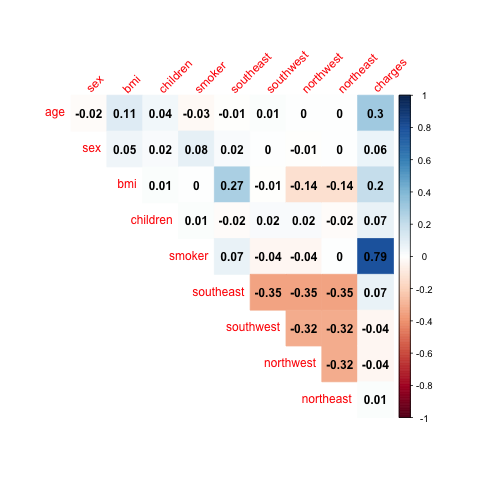
\includegraphics[width=0.75\linewidth,height=0.75\textheight]{/Users/dianalin/STAT547/group01/images/corrplot} \end{center}

\hypertarget{faceted-plot}{%
\subsubsection{Faceted Plot}\label{faceted-plot}}

Here we want to explore the data to see if there is any cluster of data
points. While the data between regions and sex does not appear to vary
much, the smokers vs nonsmokers of each facet appear to cluster
together, with the non-smokers having an overall lower medical cost.

\begin{center}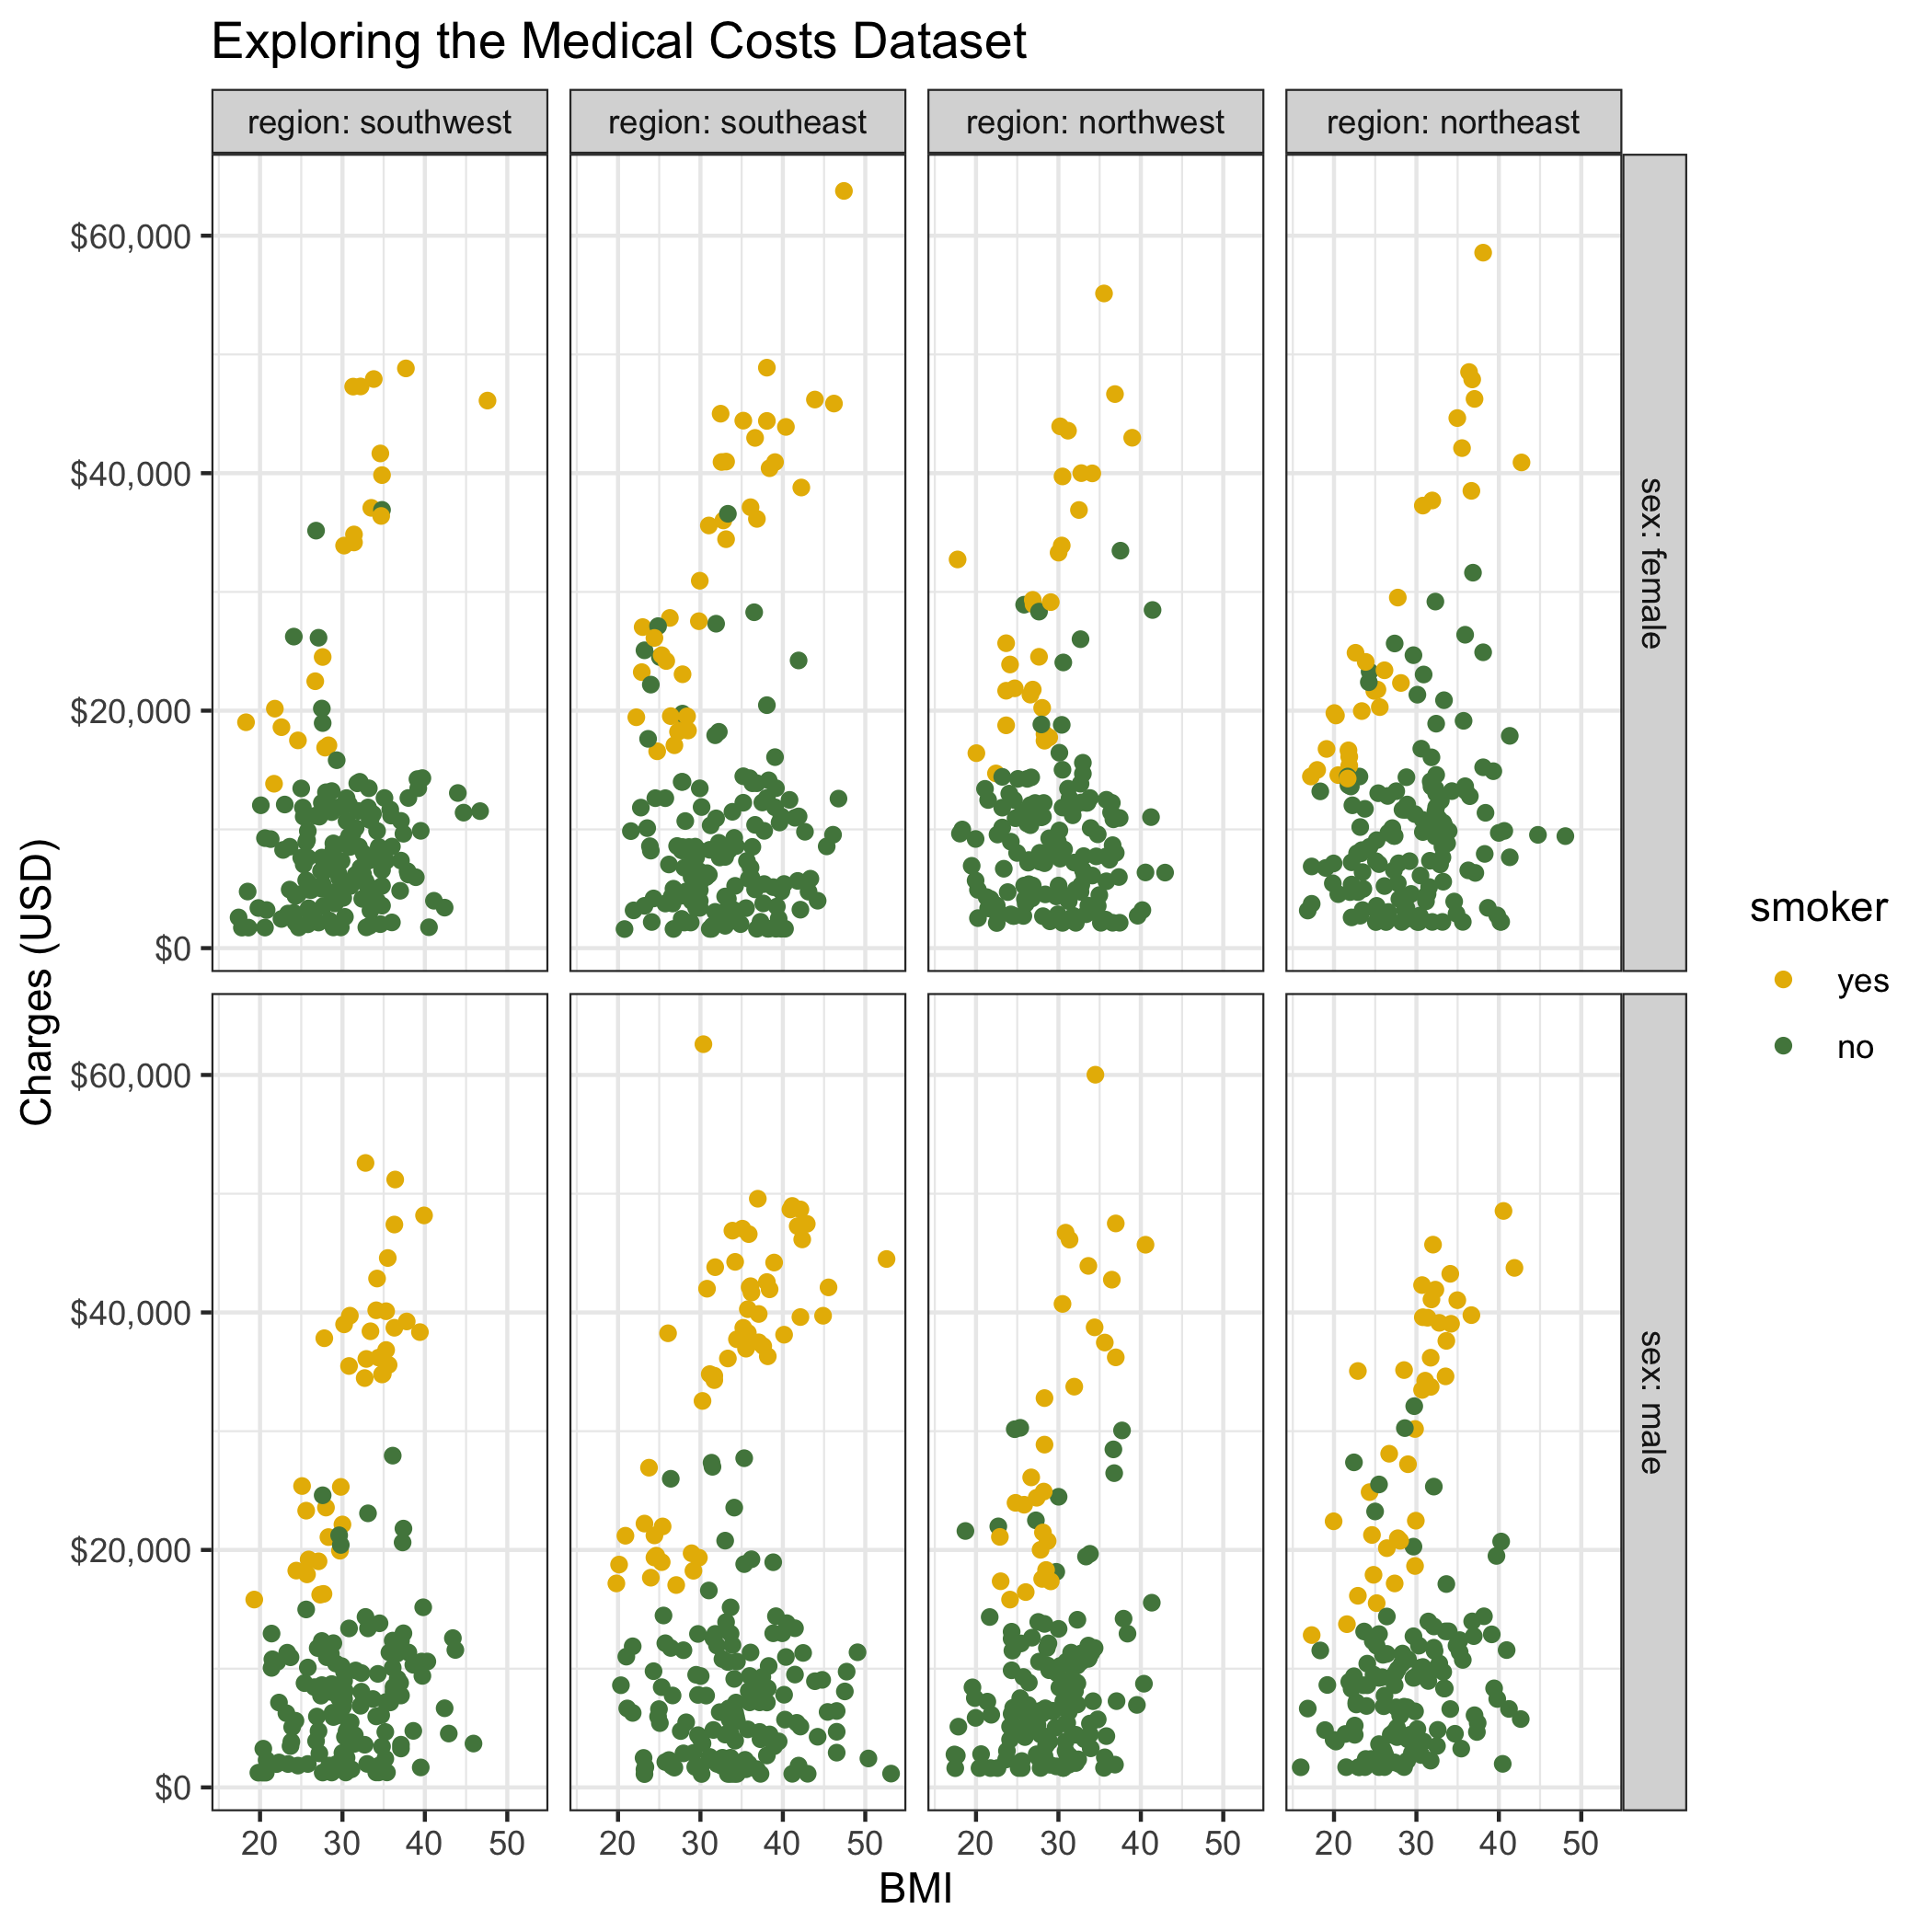
\includegraphics[width=0.75\linewidth,height=0.75\textheight]{/Users/dianalin/STAT547/group01/images/facet} \end{center}

\hypertarget{histogram}{%
\subsubsection{Histogram}\label{histogram}}

How is the distribution of sex among different age groups? Looking at
the dataset, there appears to be more beneficiaries in the 20-60 age
range. The biggest difference in the number of beneficiaries from
different sex is seen in the 20-30 bracket.

\begin{center}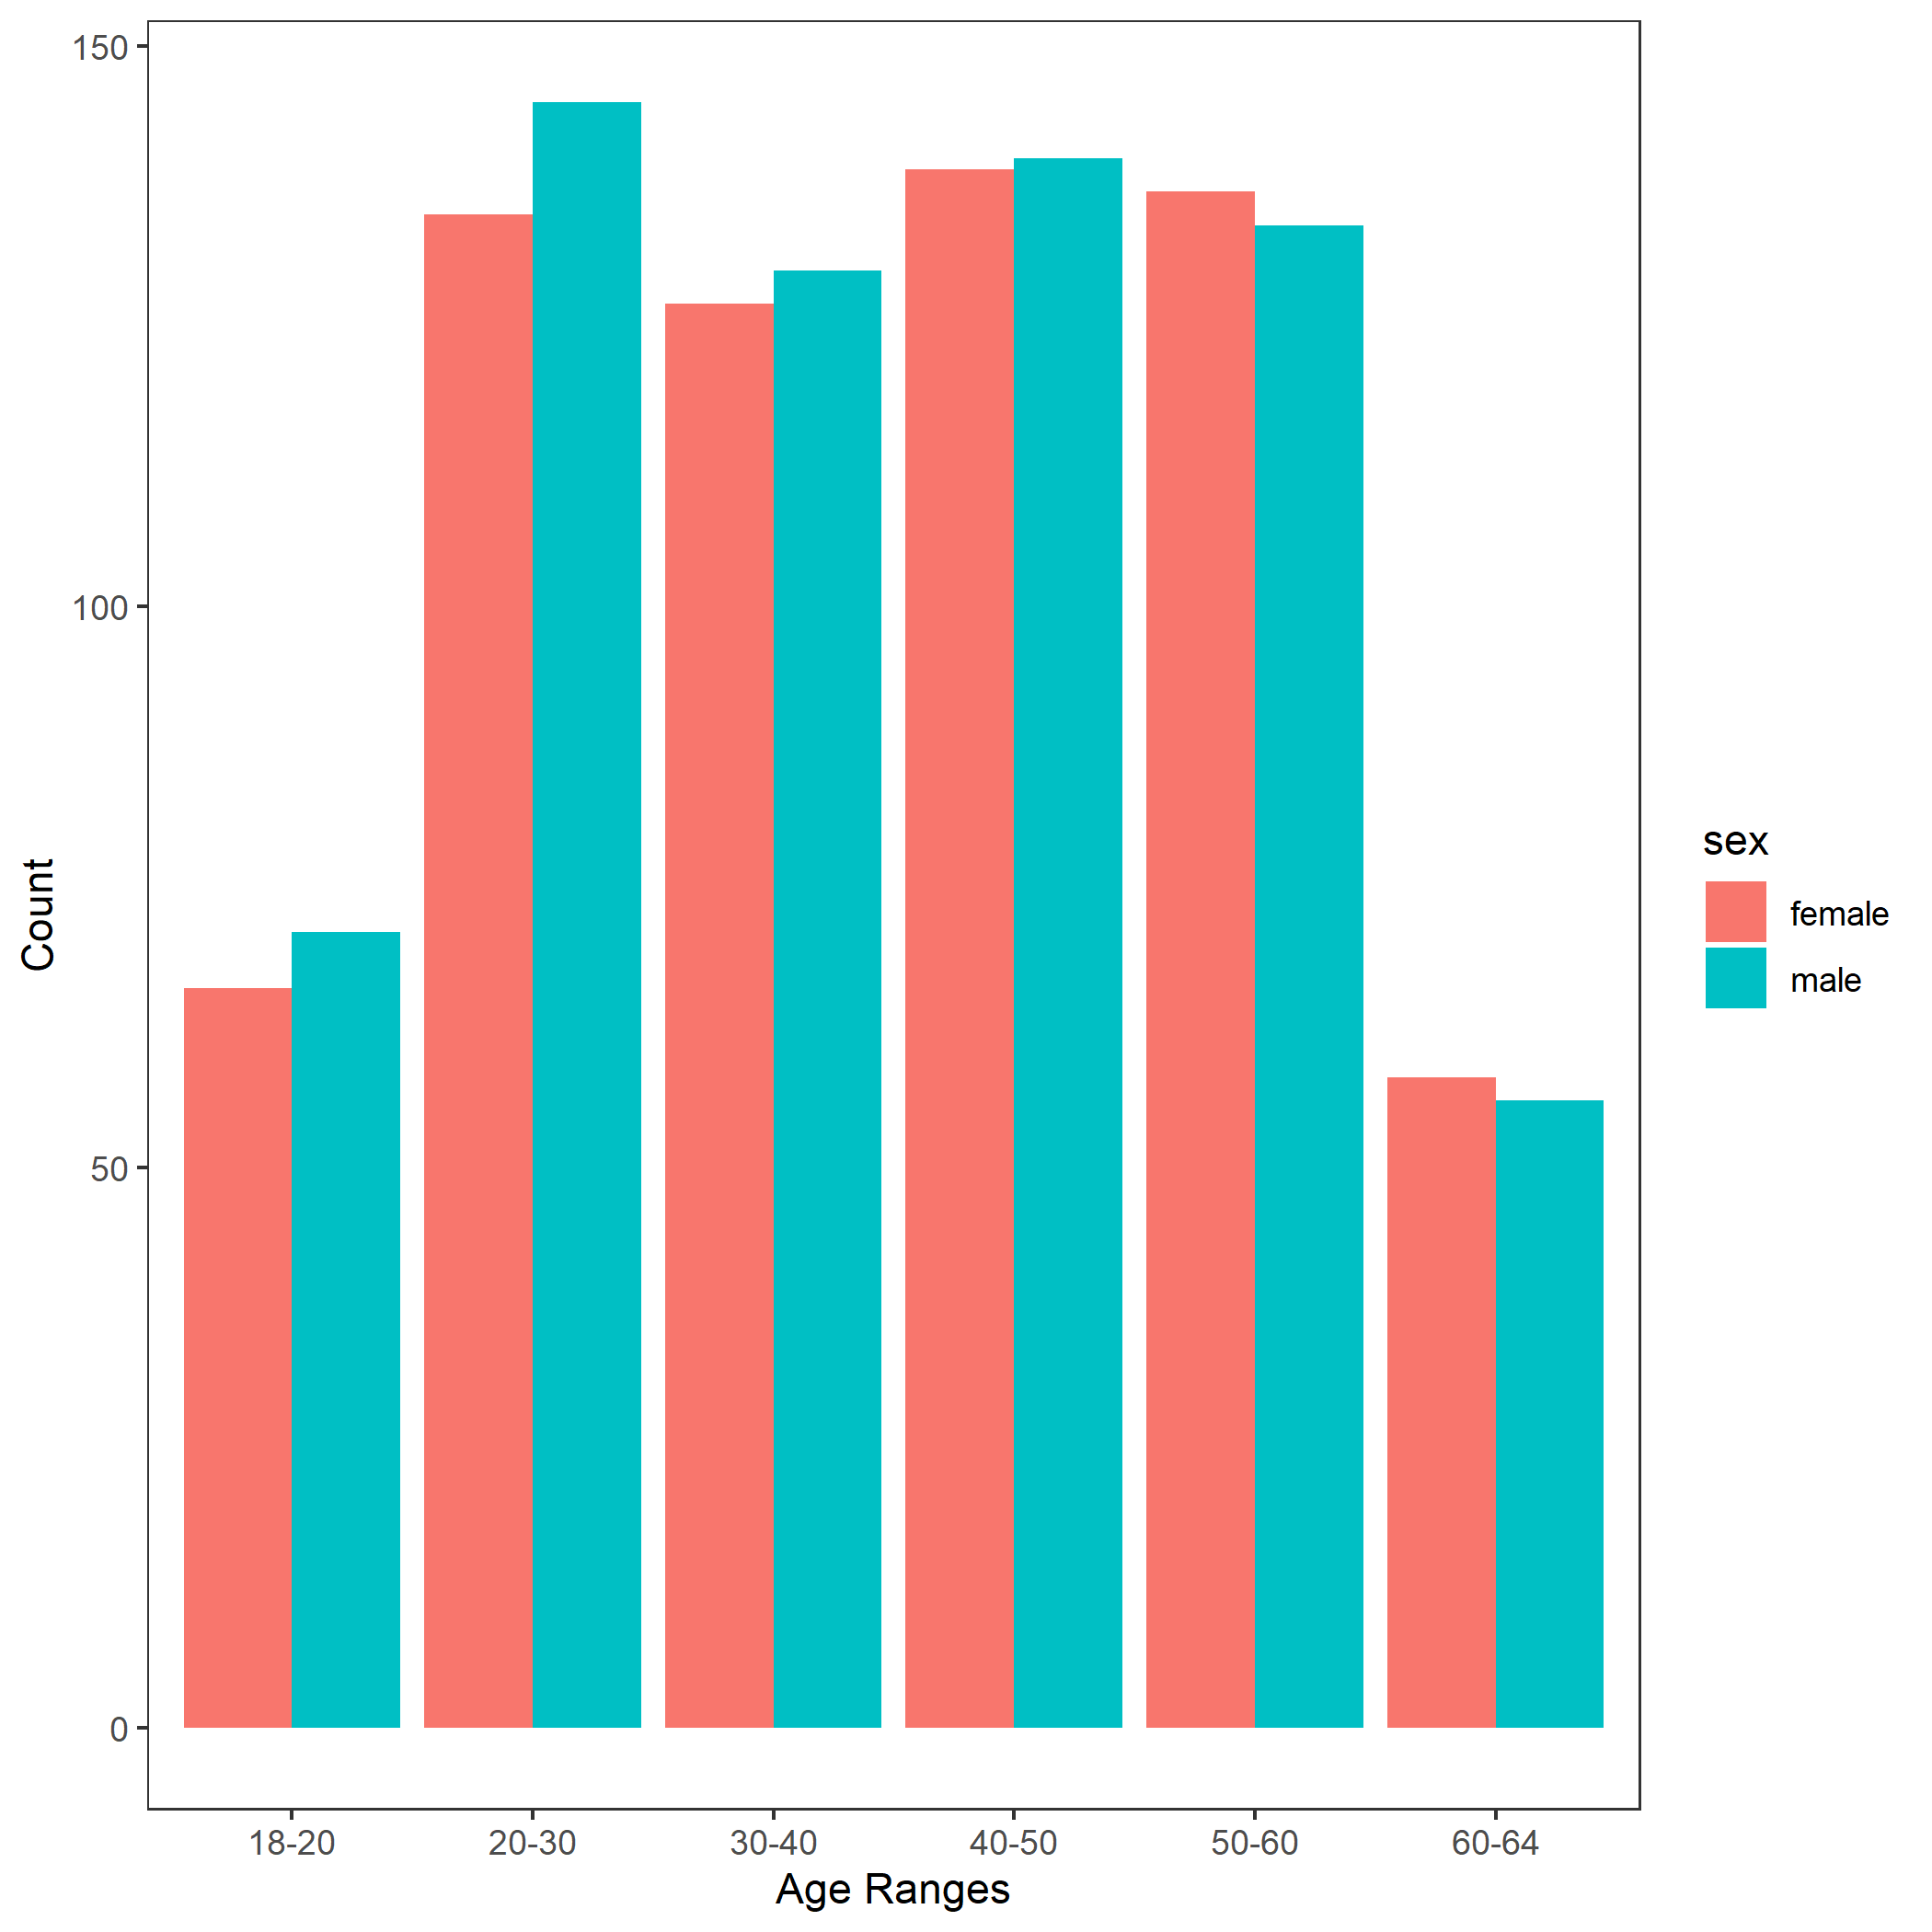
\includegraphics[width=0.75\linewidth,height=0.75\textheight]{/Users/dianalin/STAT547/group01/images/age_histogram} \end{center}

\hypertarget{stacked-bar-chart}{%
\subsubsection{Stacked Bar Chart}\label{stacked-bar-chart}}

How about the distribution of sex among the regions? This plot shows the
distribution of sex in each of the four regions. At a glance, the
dataset looks very even when it comes to sex, but there are slightly
more beneficiaries in the southeast.

\begin{center}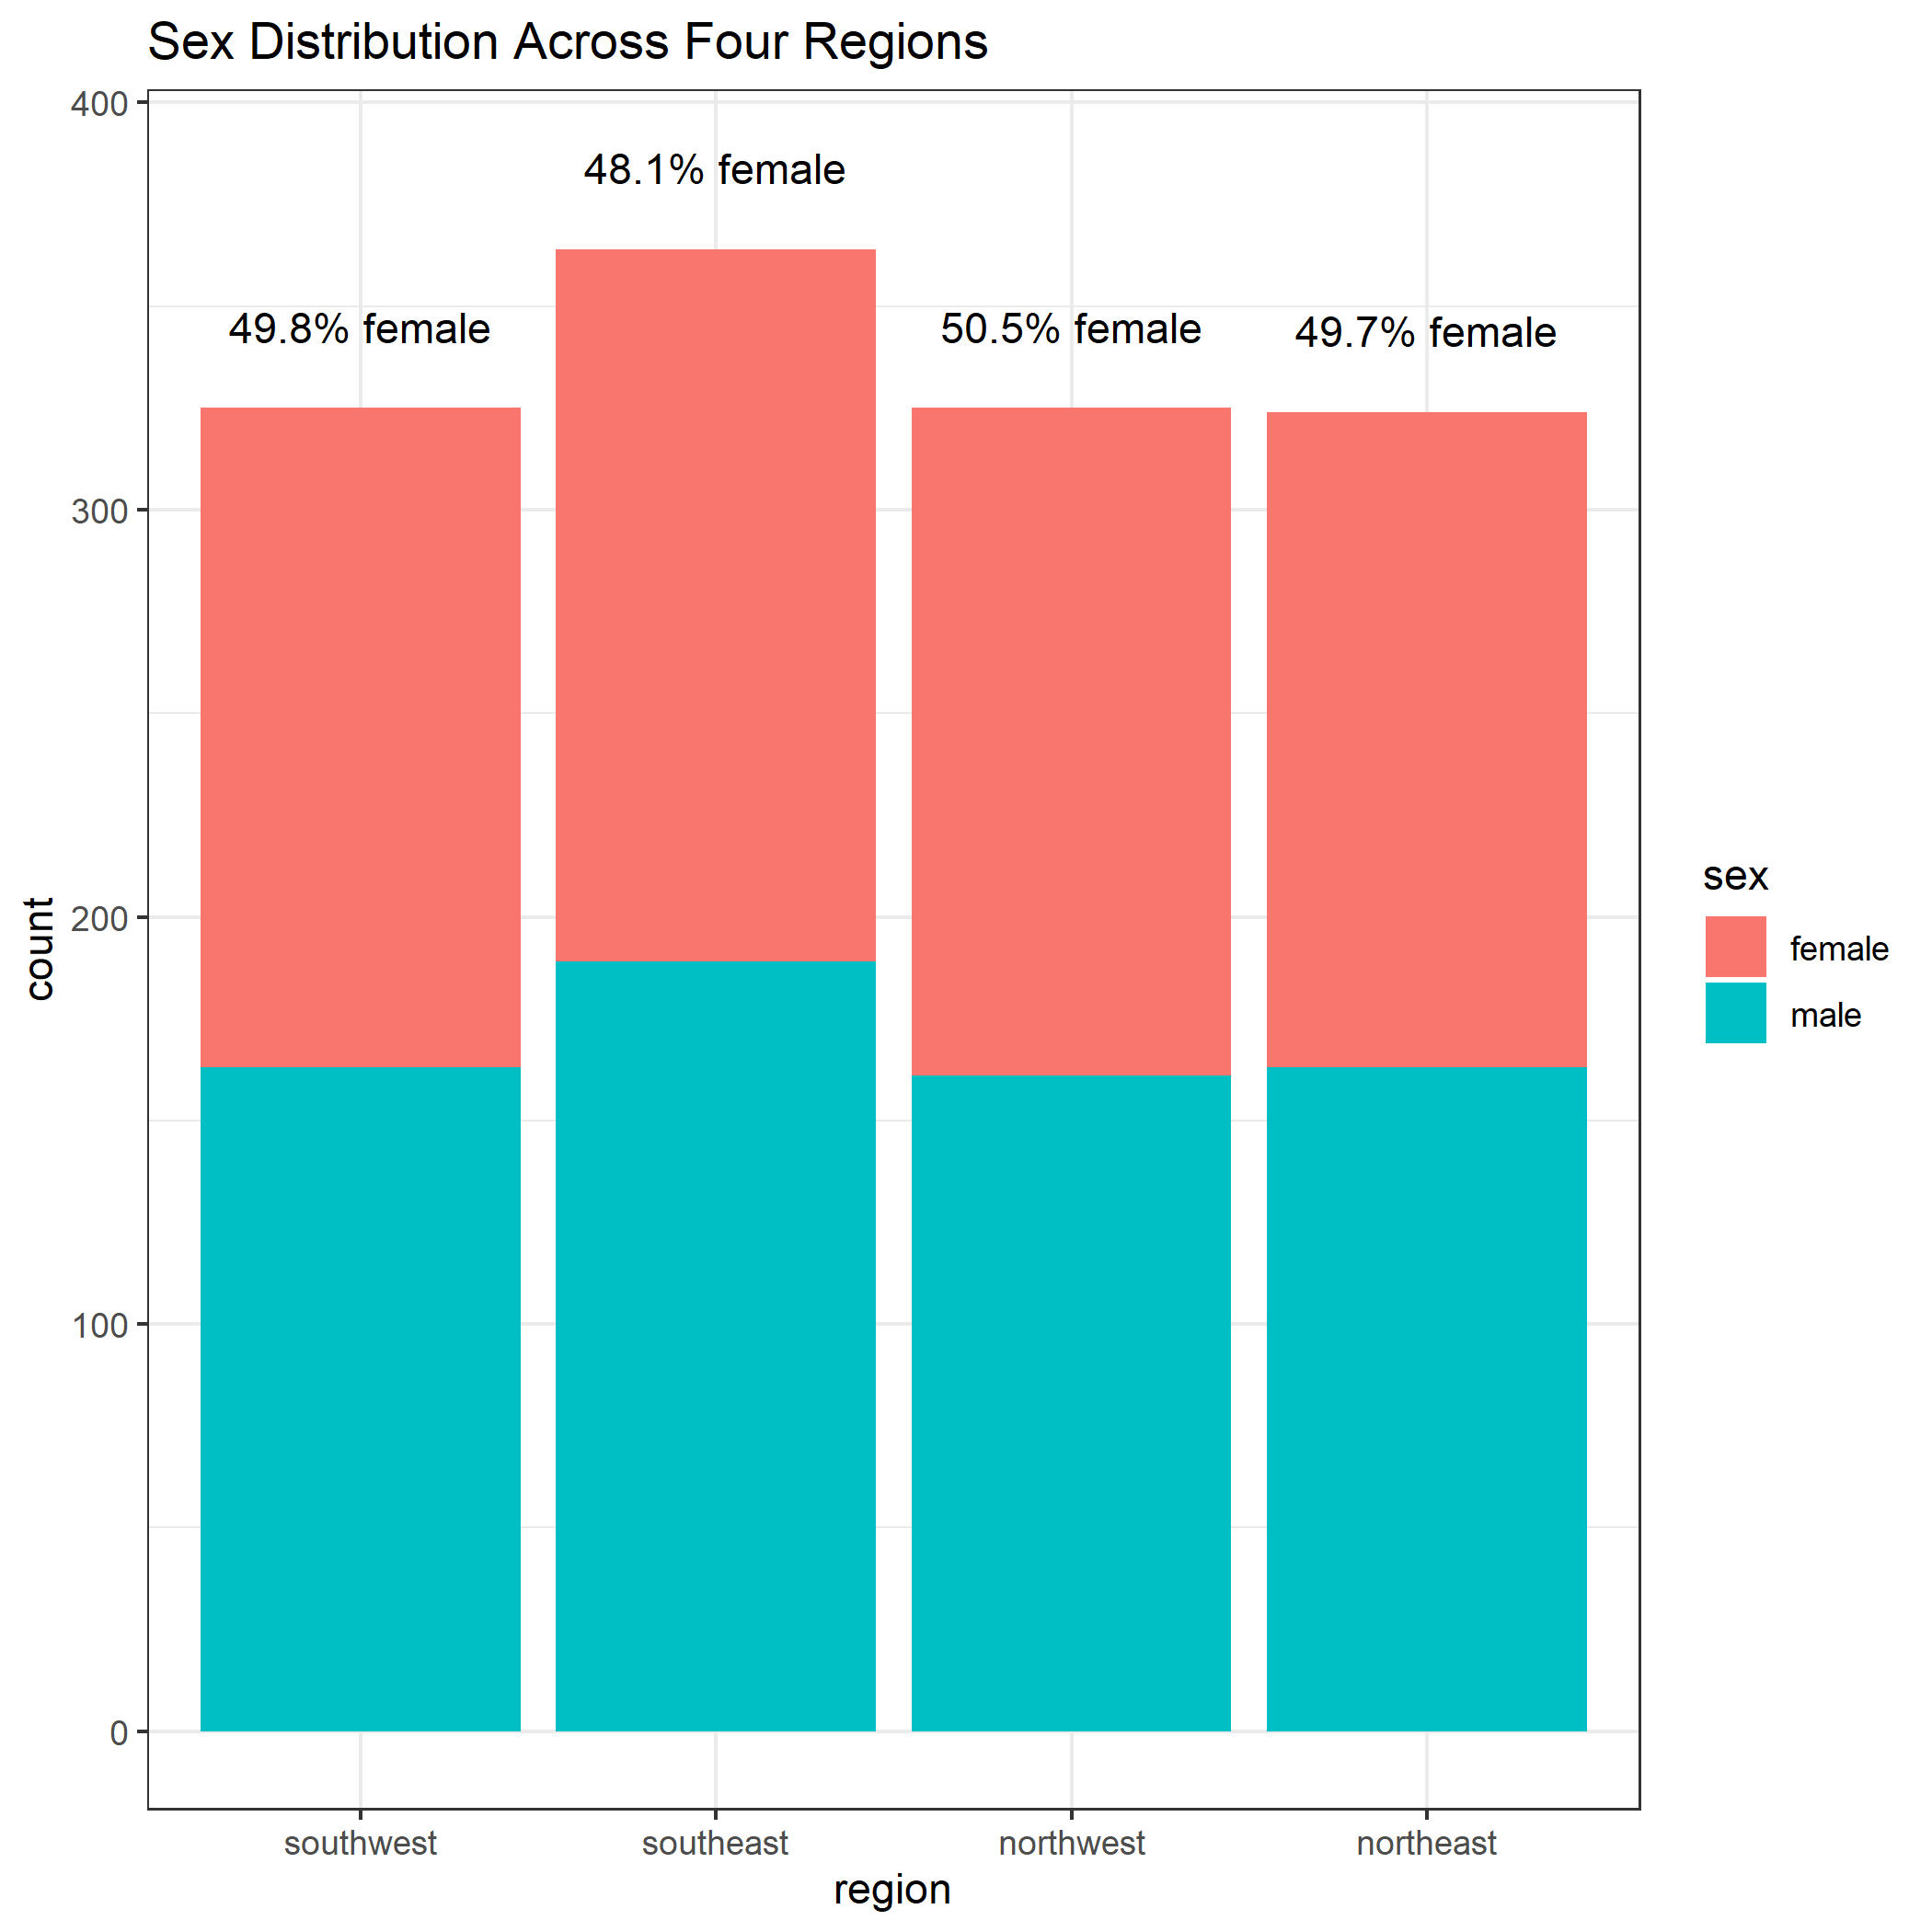
\includegraphics[width=0.75\linewidth,height=0.75\textheight]{/Users/dianalin/STAT547/group01/images/region_barchart} \end{center}

\hypertarget{methods}{%
\subsection{Methods}\label{methods}}

\begin{Shaded}
\begin{Highlighting}[]
\CommentTok{# PLACE HOLDER FOR LINEAR REGRESSION}
\end{Highlighting}
\end{Shaded}

\hypertarget{results}{%
\subsection{Results}\label{results}}

\begin{Shaded}
\begin{Highlighting}[]
\CommentTok{# PLACEHOLDER FOR LINEAR REGRESSION}
\end{Highlighting}
\end{Shaded}

\hypertarget{discussion}{%
\subsection{Discussion}\label{discussion}}

\begin{Shaded}
\begin{Highlighting}[]
\CommentTok{# PLACEHOLDER FOR LINEAR REGRESSION}
\end{Highlighting}
\end{Shaded}

\hypertarget{conclusion}{%
\subsection{Conclusion}\label{conclusion}}

\begin{Shaded}
\begin{Highlighting}[]
\CommentTok{# PLACEHOLDER FOR LINEAR REGRESSION}
\end{Highlighting}
\end{Shaded}

\end{document}
